
\documentclass[portrait,a0,final]{a0poster}

\usepackage{epsfig}
\usepackage{multicol}
%\usepackage{pstricks,pst-grad}
\usepackage{graphicx}
\DeclareGraphicsRule{.ai}{pdf}{.ai}{}
\usepackage{color}
\usepackage{tabularx}
\usepackage{multirow}
\usepackage{amssymb,amsmath,amsthm}

%%%%%%%%%%%%%%%%%%%%%%%%%%%%%%%%%%%%%%%%%%%
% Definition of some variables and colors
%\renewcommand{\rho}{\varrho}
%\renewcommand{\phi}{\varphi}
%\newrgbcolor{nus_blue}{0 0.129 0.388}IPS_2016_lijiong
%\newrgbcolor{nus_gold}{1 0.259 0}
%\newrgbcolor{nus_lite}{1 0.259 0}
%\newrgbcolor{lite}{.70 .70 .70}
%\newrgbcolor{liter}{.95 .95 .95}
\setlength{\columnsep}{3cm}
% \setlength{\columnseprule}{2mm}
\setlength{\parindent}{0.0cm}


%% Figures and tables
%% The multicols package doesn't support the floats, figure and table.
%% Use tablehere and figurehere in place of table and figure.

\makeatletter
\newenvironment{tablehere}
  {\def\@captype{table}}
  {}

\newenvironment{figurehere}
  {\def\@captype{figure}}
  {}
\makeatother


% \figcaption replaces - replacement for \caption
% necessary, since in the multicols environment \figure and
% therefore \caption won't work

\newcommand{\ket}[1]{|{#1}\rangle}
\newcommand{\bra}[1]{\langle{#1}|}
\newcommand{\braket}[1]{\langle{#1}\rangle}

\setcounter{figure}{1}
\newcommand{\figcaption}[1]{
%  \vspace{0.5cm}
  \begin{center}
  \begin{quote}
    {\large {\sc Figure} \arabic{figure}: #1}
  \end{quote}
  \end{center}
 % \vspace{1cm}
  \stepcounter{figure}
}

\setcounter{table}{1}
\newcommand{\tabcaption}[1]{
  \vspace{0.5cm}
  \begin{center}
  \begin{quote}
    {\normalsize {\sc Table} \arabic{table}: #1}
  \end{quote}
  \end{center}
 % \vspace{1cm}
  \stepcounter{table}
}
%%%%%%%%%%%%%%%%%%%%%%%%%%%%%%%%%%%%%%%%%%%%%%%%%%%%
%%%                Poster                        %%%
%%%%%%%%%%%%%%%%%%%%%%%%%%%%%%%%%%%%%%%%%%%%%%%%%%%%

\newenvironment{poster}{
  \begin{center}
  \begin{minipage}[c]{0.98\textwidth}
}{
  \end{minipage}
  \end{center}
}




%%%%%%%%%%%%%%%%%%%%%%%%%%%%%%%%%%%%%%%%%%%%%%%%%%%%%%%%%%%%%%%%%%%%%%
%%% Begin of Document
%%%%%%%%%%%%%%%%%%%%%%%%%%%%%%%%%%%%%%%%%%%%%%%%%%%%%%%%%%%%%%%%%%%%%%

\begin{document}
\begin{poster}
\large \sf

%%%%%%%%%%%%%%%%%%%%%
%%% Header
%%%%%%%%%%%%%%%%%%%%%
\begin{center}

      %%% CQT_Logo
      \begin{minipage}[c]{0.05\textwidth}
        \begin{center}
          
\includegraphics[width=14cm,angle=0]{figures/CQT_Logo}
        \end{center}
      \end{minipage}\hspace{10cm}
      %%% Title
      \begin{minipage}[c]{0.7\textwidth}
        \begin{center}
          {\sc \huge
          Photon number and timing resolution of a near-infrared continuous-wave source with a transition edge sensor}\\[9mm]
          {\large Jianwei Lee$^1$,
          Lijiong Shen$^{1,2}$,
          Alessandro~Cer\`e$^1$,
          and Christian~Kurtsiefer$^{1,2}$}\\[9mm]
          {$^1$Centre for Quantum Technologies, National University of Singapore, Singapore\\
           $^2$Department of Physics, National University of Singapore, Singapore}
        \end{center}
      \end{minipage}
      %%% NUS-Logo
      \begin{minipage}[c]{.1\textwidth}
        \begin{center}
          
\includegraphics[width=8cm,angle=0]{figures/NUS_Logo.pdf}
        \end{center}
      \end{minipage}
\end{center}

\vspace{0.2cm}



%%%%%%%%%%%%%%%%%%%%%
%%% Content
%%%%%%%%%%%%%%%%%%%%%
\begin{center}
  % \begin{center}{\bf \Large \textsf {Introduction}}\end{center}
\end{center}
    The Transition Edge Sensor (TES) is a calorimetric spectrometer that have near unit efficiency and is photon-number resolving.
    %
    Slow recovery time, on the order of microseconds, limits the number resolving and timing accuracy for high photon-flux detection.
    %
    One method uses the differentiated TES signal to determine the arrival time of overlapping signals and to count X-ray photons~\cite{Fowler:2015ef}.
    %
    For near-infrared (NIR) photons the signal-to-noise ratio is low, and timing accuracy is affected by the bandwidth limitations necessary to reject false positives.
    %
    Here, we use a two-level discriminator to locate pulses, and the area of the identified signal regions to count photons.
    %
    We show how it
    improves photon number discrimination for NIR continuous wave (CW) sources,
    and propose a scheme to determine the arrival time and pulse amplitude of the underlying pulses.

\begin{multicols}{2}
\setlength{\parskip}{0ex}
% %!TEX root =  pulse_fitting_poster.tex
\vspace{-1cm}
\begin{center}
  \begin{center} {\bf \Large \textsf {Motivation}}\end{center}
\end{center}
Standard techniques for time-tagging a detection event, based on threshold crossing or constant fraction discrimination, do not work when two pulses have a large overlap, limiting the applicability of the TES for high photon-flux detection.
%
Previously, differentiation was used to locate the steep rising edge of individual X-ray detection events when the signals overlap~\cite{Fowler:2015ef}.
%
The number of rising edges was used
to identify the number of detected photons.
%
For near-infrared (NIR) photons the signal-to-noise ratio is lower, and timing accuracy is affected by the bandwidth limitations necessary to reject false positives.
%
In this work, we estimate the arrival time using a two-level discriminator that is inherently robust against noise.
We show how it
improves photon number discrimination for NIR continuous wave (CW) sources,
and propose a scheme to determine the arrival time and pulse amplitude of the underlying pulses.
%!TEX root =  pulse_fitting_poster.tex
% \vspace{-1cm}

\begin{center}
  \begin{center} {\bf \Large \textsf {Pulse-Region Identification}}\end{center}
\end{center}

To identify
photodetection events
we use
the digital equivalent of SET-RESET edge detection,
with SET triggered when the signal passes threshold~$V_{th}$
and RESET by the first subsequent zero crossing.
\begin{figurehere}
  \begin{center}
    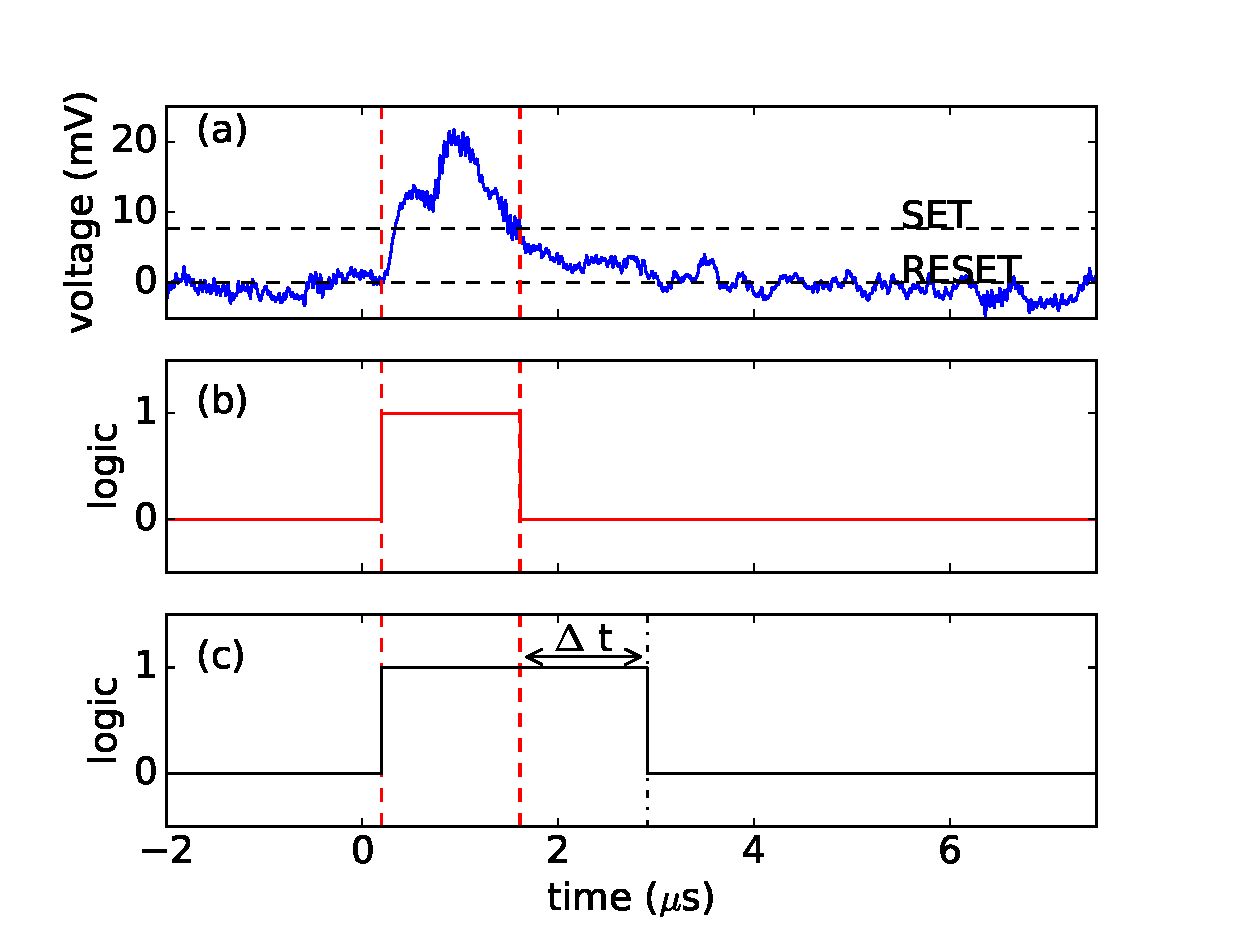
\includegraphics[width=1\linewidth]{figures/comparator/comparator_at_500ns.eps}
  \end{center}
  \vspace{-0.8cm}
  \figcaption{
	Blue trace: Overlapping pulses separated by 482~ns. The rising edge of the later pulse is obscured by the earlier pulse and prevents arrival time estimation using the threshold crossing-time.
    Red line: The two-level (discriminator) identifies the region corresponding to photon detection.
    Black line: The discriminator logic extended by $\Delta t$ to include the decaying pulse tail. This mode is used to determine the pulse area.
}
\end{figurehere}
\vspace{1cm}
We implement the SET-RESET latch backwards in time (see Fig.1).
We use this region to initialise a fit of the signal to a model to determine the pulse arrival times. 
The logic identifies the region containing the rising edges of underlying pulses,
and excludes much of the decaying tail.
In this way, we minimise the false identification of noise fluctuations along the decaying tail as photodetection events.

To determine the number of detected photons, we calculate the pulse area.
To increase signal-to-noise ratio, we extend the discriminated region by $\Delta t=1300$~ns so that the decaying tail is included. 


\begin{center}
  \begin{center} {\bf \Large \textsf {Discriminator Initialisation}}\end{center}
\end{center}

\begin{figurehere}
    \begin{center}
    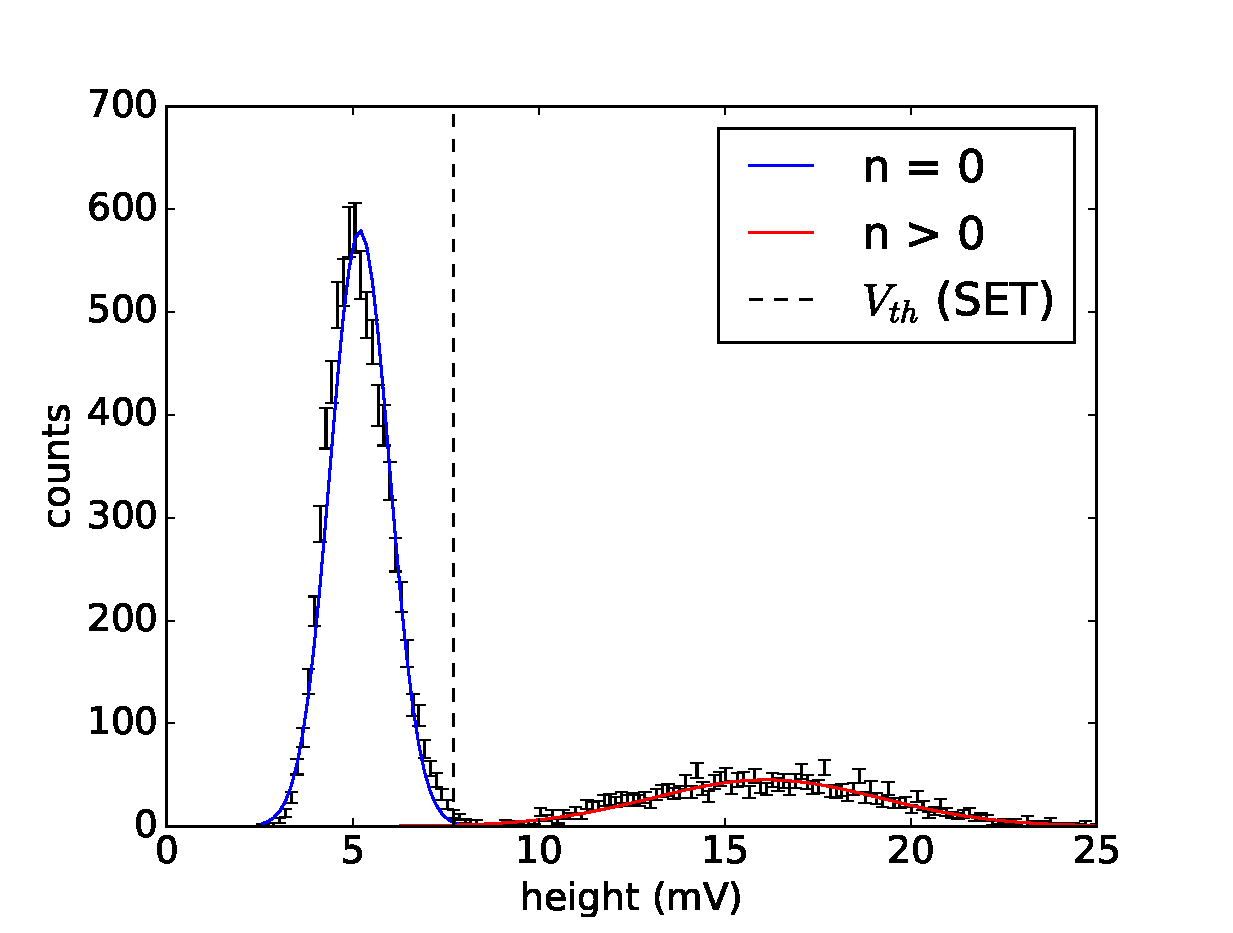
\includegraphics[width=0.9\linewidth]{figures/height_histogram_cw/height_histo.eps}
    \figcaption{\label{fig:height_histo}
        Pulse height histogram of the TES response to a continuously running LD with~$\bar{n} = 0.25$. The two peaks correspond to 0 and at least 1 photon being detected respectively. Error bars indicate Poissonian standard-deviation.
        Black line: Point of minimal overlap between Gaussian fits to the two height distributions corresponding to $V_{th} = 7.7$~mV. This threshold is used to initialise the SET-RESET discriminator.}
    \end{center}
\end{figurehere}
 %\\[1cm]
\columnbreak
%!TEX root =  pulse_fitting_poster.tex
\begin{center}
  \begin{center} {\bf \Large \textsf {Photon Number Discrimination}}\end{center}
\end{center}

To determine the number of photodetection events, we calculate the signal area and assume that it is proportional to the energy absorbed~\cite{Cabrera2000509}.

To increase signal-to-noise ratio, we use the discriminator 
to identify integration windows surrounding pulses 
that exhibit a leading edge and decaying tail (Fig.1c).

In this way, pulses that are partially captured within our finite acquisition windows ($10~\mu$s) do not degrade the pulse-integral distinguishability between traces containing complete photodetection events.

We compute the pulse area $a$ for every trace
and organize them in histogram $C(a)$.

\begin{figurehere}
  \begin{center}
	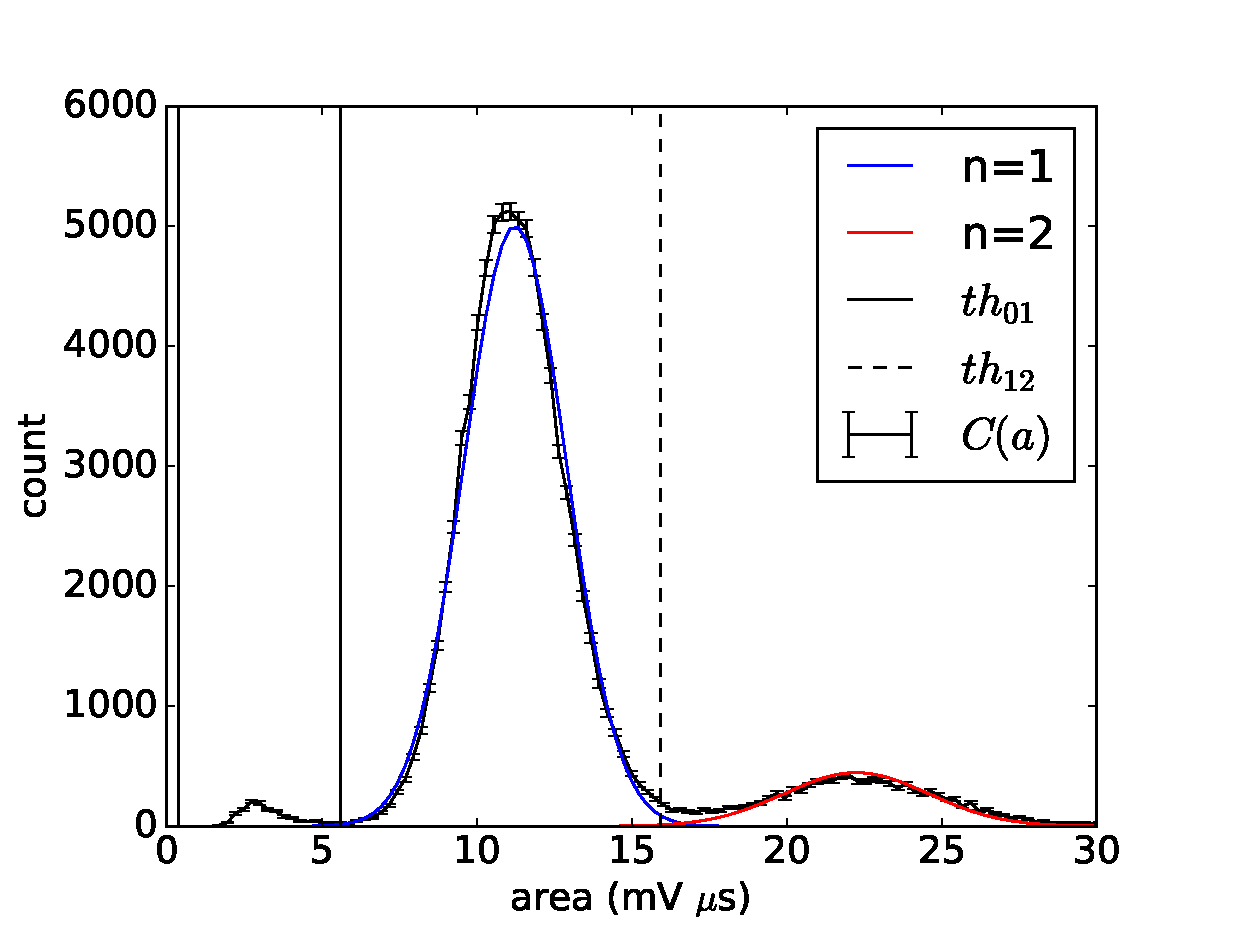
\includegraphics[width=0.9\linewidth]{figures/area_histogram_cw/area_histo_with_fit.eps}
  \end{center}
  % \vspace{-2cm}
  \figcaption{\label{fig:area_histos_comparison}
        Pulse area distribution $C(a)$ of the signal in the discriminated region.  
        The first bin ($a = 0$) corresponds to zero photodetection events being discriminated.
        The small distribution to the left of $th_{01} = 5.6$~mV$\,\mu$s corresponds to traces with detector noise exceeding $V_{th}$.
        The minimum of $C(a)$ between the $n=0$ and $n=1$ distribution corresponds to the threshold $th_{01}$.
        % Equally separated peaks corresponding to 1, 2, 3 and 4 photons demonstrates the linear dependence of the area with photon energy. 
        Error bars indicate Poissonian standard-deviation.
    }
 %    \figcaption{\label{fig:area_histos_comparison}
 %    The pulse area distribution obtained with the discriminator 
	% improves resolution: Red Line: area distribution of entire trace. Green line: area distribution of signal above $V_{th}$. Blue line: area distribution $C(a)$ of the signal region identified using the discriminator described in section~\ref{sec:disc}. Vertical lines: area thresholds $th_{mn}$ separating $m$ and $n$-photon events identified by the discriminator.
 %    }
\end{figurehere}
% \vspace{1cm}
We fit the area distribution 
identified by the discriminator 
corresponding to $n>0$ detection events 
to a linear combination of Gaussian distributions~
$G_1(a; a_1, \sigma_1)$ and $G_2(a; a_2, \sigma_2))$.

% \vspace{1cm}
% The ratio of the peak positions $a_2/a_1 = 1.98$ demonstrates the linear dependance of the pulse area with photon energy.

At the minimum overlap between the distributions $th_{12}$,
the probability of falsely identifying an $n=1$ trace as an $n=2$ trace is 0.2\%,
while
the probability of falsely identifying an $n=2$ trace as an $n=1$ trace is 0.3\%.
\vspace{1cm}
%
% We calibrate the detector by classifying a trace 
% with area $a \in [a_n-2\,\sigma_n,a_n+2\,\sigma_n]$ as an $n$-photon event.
%
% We determine the minimum overlap between $G_1(a; a_1, \sigma_1)$ and $G_2(a; a_2, \sigma_2)$ to be the threshold $th_{12}$. 
% At this threshold, 
% the probability of falsely identifying an $n=1$ trace as an $n=2$ trace is 0.2\%,
% while
% the probability of falsely identifying an $n=2$ trace as an $n=1$ trace is 0.3\%,
%!TEX root =  pulse_fitting_poster.tex
\begin{center}
  \begin{center} {\bf \Large \textsf {Outlook: Arrival Time Estimation}}\end{center}
\end{center}
% We demonstrated a technique that counts photons using the area of a signal portion identified with a discriminator. 
% This technique is a useful alternative to identifying the number of pulse edges using differentiation, especially when signal-to-noise ratio is small.
% \vspace{1cm}
As an extension to this technique, we use the discriminator region (Fig.1b) to bound the range of values expected for the arrival time of individual pulses in a trace containing $N$ overlapping signals. 
%
We use this bound to initialise a least-squares fit of the signal to a multi-photon model comprising of a linear superposition of $N$ single-photon models.
%
The fit returns the amplitudes and arrival times of the individual pulses.
%
\begin{figurehere}
  \begin{minipage}{0.7\linewidth}
    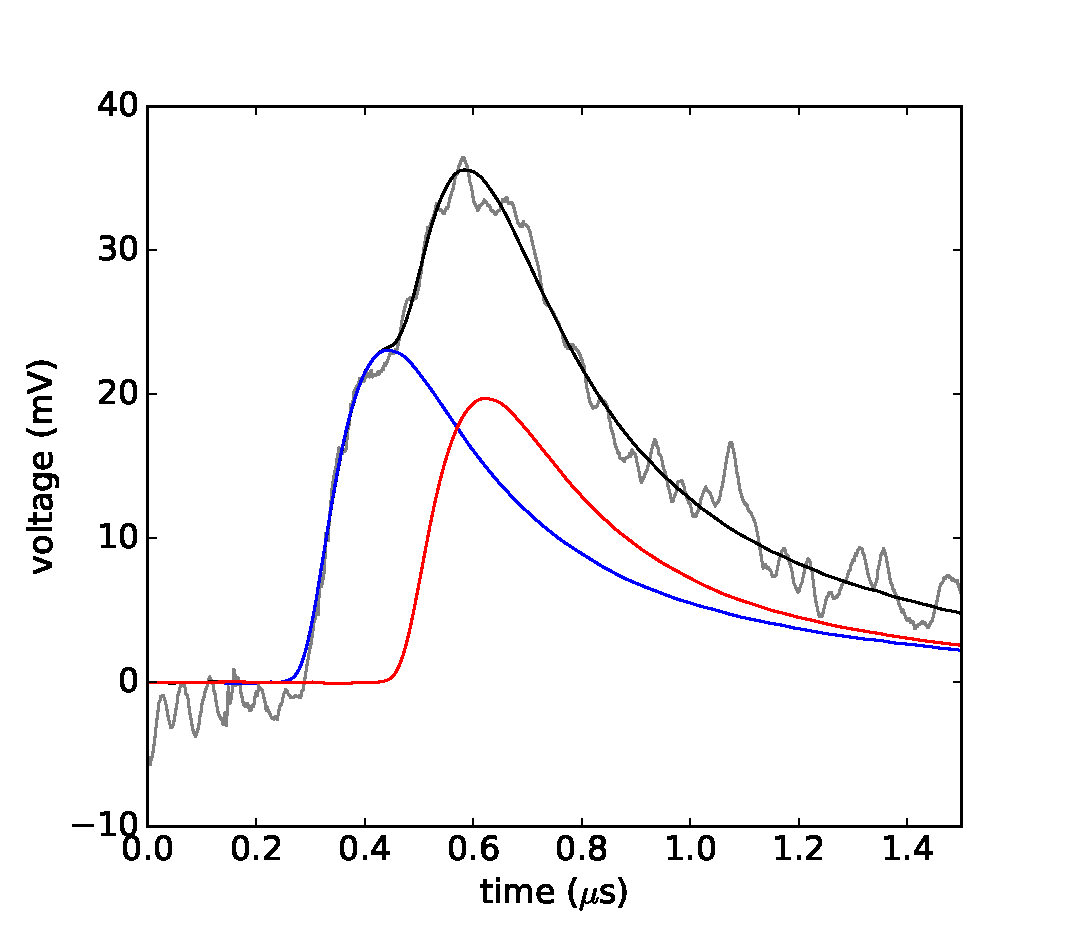
\includegraphics[width=1\linewidth]{figures/mcmc_components_170ns/mcmc_fitted_components_170ns.eps}
  \end{minipage}
  \begin{minipage}{0.3\linewidth}

    \figcaption{\label{fig:height_histo}
    Fit (black) of a 2-photon signal (grey) composed of individual single photon events (red, blue) separated by ~$\sim$170~ns, comparable to twice the rise time of a single photon pulse. 
    %
    The single photon model was obtained by averaging the TES response to 300 single photon events.
}
  \end{minipage}
\end{figurehere}
% \input{rnd_poster_fast_switch}
% \input{rnd_poster_outlook}
% \input{rnd_poster_bib}
\end{multicols}

\begin{center}{\bf \large \textsf {References}}\end{center}

\begin{multicols}{2}
  {\small
  \begin{flushleft}
  \noindent
  % \newline
  [1] J.~S.~Bell,
    % ``On the Einstein Podolsky Rosen paradox,'',
    Physics  \textbf{1}, 195 (1964).
  \newline
  ~[2] B.~Hensen, \textit{et al.},
    % ``Loophole-free Bell inequality violation using electron spins separated by 1.3 kilometres'',
    Nature \textbf{526}, 682 (2015).
  \newline
  ~[3] M.~Giustina, \textit{et al.},
    % ``Significant-Loophole-Free Test of Bell’s Theorem with Entangled Photons'',
    Phys. Rev. Lett. \textbf{115}, 250401 (2015).
  \newline
  ~[4] L. K. Shalm, \textit{et al.}
    % ``Strong Loophole-Free Test of Local Realism'',
    Phys. Rev. Lett. \textbf{115}, 250402 (2015).
  \newline
  ~[5] S. Pironio, \textit{et al.},
    % ``Random Numbers Certified by Bell's Theorem'',
    Nature \textbf{464}, 1021 (2010).
  \newline
  ~[6] M.~Fiorentino, \textit{et al.},
    % ``Generation of ultrabright tunable polarization entanglement without spatial, spectral, or temporal constraints'',
    Phys. Rev. A \textbf{69}, 041801 (2004).
  \newline
  ~[7] P. H.~Eberhard,
    % ``Background level and counter efficiencies required for a loophole-free Einstein-Podolsky-Rosen experiment'',
    Phys Rev. A \textbf{47}, R747 (1993)
  \newline
  ~[8] A.~E.~Lita, A.~J.~Miller, S.~W.~Nam,
    % ``Counting near-infrared single-photons with ($>$ 95\%) efficiency'',
    Optics express \textbf{16}, 3032 (2008).
  \newline
  % ~[9] E.~Knill, Nature \textbf{409}, 46-52 (2001). %[1]
  % \newline
  % [2] P.~H.~Eberhard, Phys. Rev. A \textbf{47}, R747 (1993).
  % \newline
  % [3] M.~Giustina et al., Nature \textbf{497}, 227 (2013).
  % \newline
  % [4] J.~S.~Bell, Physics \textbf{1}, 195-200 (1964).
  % \newline
  ~[9] R.~Colbeck, PhD Thesis University of Cambridge (arXiv:0911.3814), (2006). %[5]
  \newline
  % [2] B. Hensen et al., Nature \textbf{526}, 682 (2015).
  % \newline
  % [6] M.~Fiorentino et al., Phys. Rev. A \textbf{69}, 041801 (2004). 
  % \newline
  % ~[10] J.~D.~Bancal et al., New Journal of Phys. 16 (2014) 033011. %[7]
  % \newline
  ~[10] W.~P.~Grice, Phys. Rev. A \textbf{84}, 042331 (2011).
  \newline %[8]
  % [9] A.~E.~Lita et al., Opt. Express \textbf{16},3032 (2008).
  % \newline
  ~[11] A.~L.~Linares et al., Appl. Phys. Lett. \textbf{102}, 12117 (2013). %[10]
  \newline 
  ~[12] S.~W.~Lee et al., Proc. of the First Int. Workshop on ECS, 41-46, (2013). %[11]
  \newline 
  % \newline
  % ~[6] W.P.~Grice,
  %   ``Arbitrarily complete Bell-state measurement using only linear optical elements'',
  %   Phys. Rev. A, \textbf{84}, 042331 (2011).
  % \newline
  ~[13] B.~Williams et al., 
  % "Complete Bell state measurement realized utilizing time-polarization hyperentanglment," 
  Conference on Lasers and Electro-Optics, 
  % OSA Technical Digest (online) 
  % Optical Society of America, 
  \textbf{FM2N.8}, (2016).
  \end{flushleft}
  } 
\end{multicols}

\end{poster}
\end{document}
